\chapter*{Introduzione}

Questo progetto è ispirato ad un lavoro del 2018 intitolato 
\textit{``Super SloMo: High Quality Estimation of Multiple Intermediate Frames for Video Interpolation''}
(disponibile a \href{http://jianghz.me/projects/superslomo/}{questo link}).
Tale studio illustra l'uso di reti neurali convoluzionali (CNN) per svolgere l'\textit{interpolazione dei frame} 
in un video.

Lo scopo del progetto era quello di realizzare un'applicazione Android che implementasse un sistema di slow motion 
"artificiale" tramite le tecniche esposte nell'articolo sopra citato. In particolare, è stata utilizzata 
un'implementazione del modello in Pytorch disponibile su GitHub, la quale è stata adattata per l'utilizzo su un 
dispositivo Android.

\section*{Interpolazione dei frame}

Una delle tecniche tradizionali per realizzare video in slow-motion risiede nell'utilizzo di telecamere capaci di 
registrare video a framerate elevati, ad esempio 240 fps (tuttavia in casi con esigenze particolari si possono 
raggiungere anche decine di migliaia di fps). In questo modo è possibile poi rallentare il video, riproducendolo ad 
un framerate più basso (tipicamente 25-30 fps) e ottenendo quindi un effetto slow-motion.

Nel contesto dei dispositivi embedded, tuttavia, può essere impossibile equipaggiare telecamere di questo tipo (per via
dei costi o delle dimensioni). In questi casi risulta utile disporre di strategie alternative, come l'interpolazione dei 
frame. Questa tecnica, applicata ad un video pre-registrato, mira a generare artificialmente uno o più fotogrammi intermedi 
a partire da due fotogrammi consecutivi, al fine di aumentare il framerate del video e consentire di riprodurlo in slow-motion
successivamente mantenendone la fluidità. Ovviamente, questo metodo garantisce una precisione molto inferiore rispetto
all'utilizzo di telecamere ad alta velocità, essendo i frame aggiuntivi ottenuti tramite una stima e non effettivamente
catturati dalla telecamera.

L'interpolazione dei frame può essere implementata in diversi modi, l'implementazione che verrà utilizzata in questo progetto
è basata su reti neurali convoluzionali, come già anticipato. Di seguito un confronto dei risultati ottenuti con diverse
implementazioni, estratto dal paper di riferimento.

\newpage

\begin{figure}[t!]
    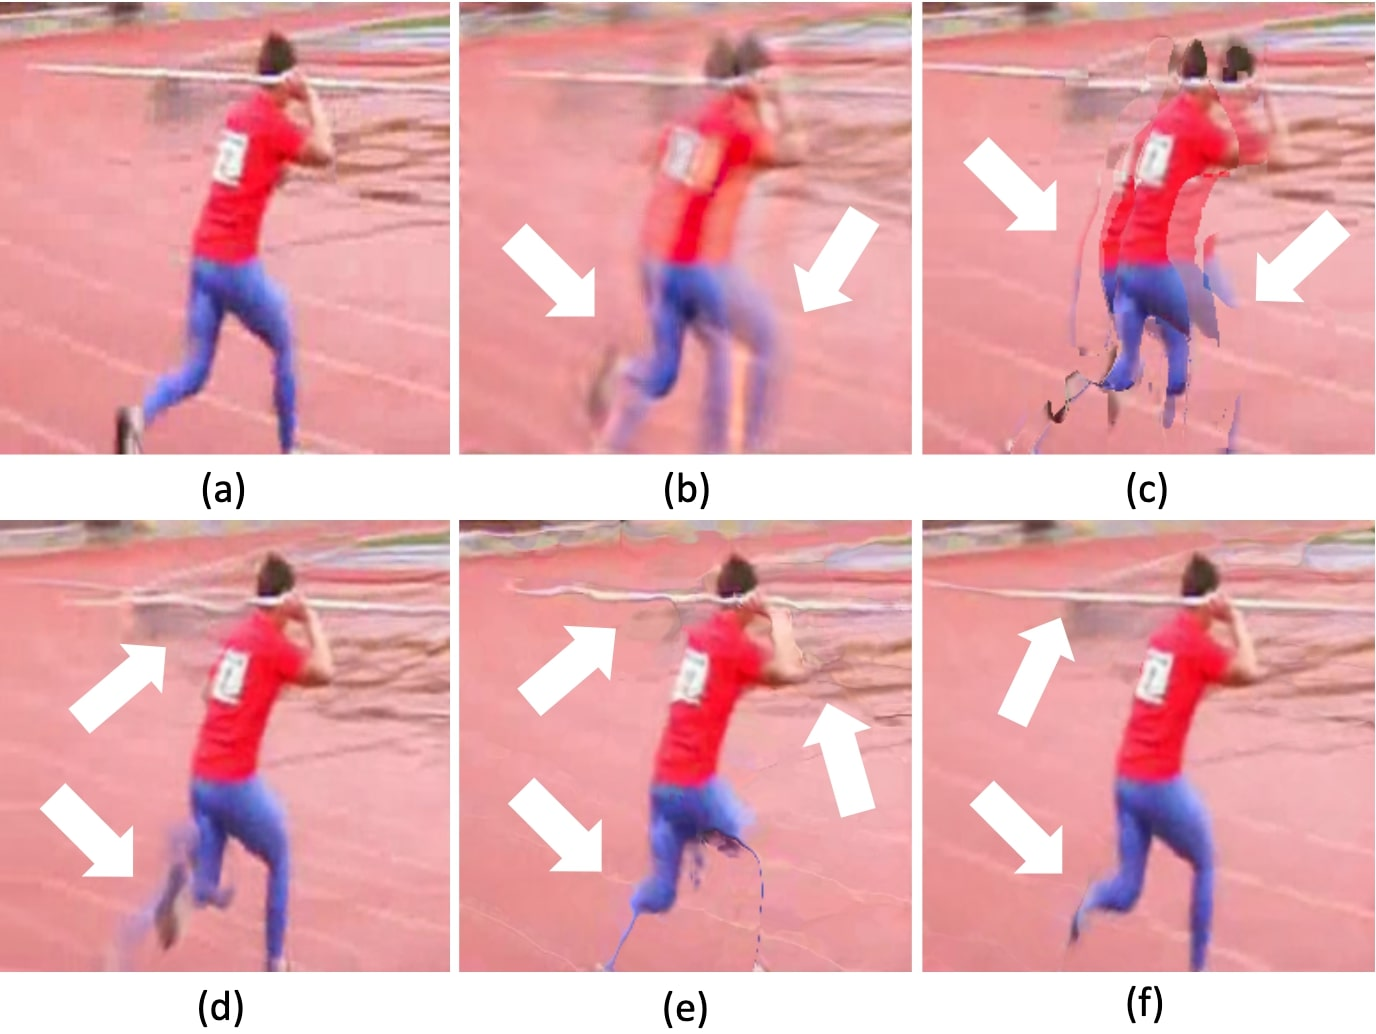
\includegraphics[width=0.7\textwidth]{img/confronto_interpolazione_frame.jpg}
    \centering
    \caption{(a) frame intermedio originale; risultati di interpolazione con: (b-e) diverse implementazioni, (f) implementazione
    di riferimento. Fonte: https://arxiv.org/abs/1712.00080}
    \label{fig:confronto_interpolazione_frame}
\end{figure}

Nel successivo capitolo si procede a descrivere brevemente il modello Pytorch utilizzato, alcune sue caratteristiche
e il processo di conversione necessario per l'utilizzo su dispositivo Android.